%<dscrpt>Introduction aux anneaux quadratiques.</dscrpt>
L'objet de ce problème\footnote{d'après Algebraic Number Theory, I.N. Stewart \& D.O. Tall (Chapman and Hall)} est d'explorer quelques propriétés de sous-anneaux de $\R$ ou de $\C$ notés $\Z[\alpha]$ définis par 
\begin{displaymath}
  \Z[\alpha] = \left\lbrace a + b\alpha , (a,b)\in \Z^2 \right\rbrace 
\end{displaymath}
où $\alpha \in \C \setminus \Q$ est solution d'une équation du second degré à coefficients entiers.\newline
On considèrera par exemple $\Z[i]$ (entiers de Gauss) comme cas particulier des $\Z[i\sqrt{d}]$ ou $\Z[\sqrt{d}]$ pour divers entiers naturels $d$ ainsi que $\Z[j]$ où $j=e^{\frac{2i\pi}{3}}$ est une racine troisième de l'unité ou encore $\Z[\varphi]$ où $\varphi$ est le \emph{nombre d'or} c'est à dire le réel positif vérifiant $\varphi^2 = \varphi + 1$.
\subsection*{I. Préliminaires}
Soit $\alpha \in \C \setminus \Q$ pour lequel il existe $p$ et $q$ entiers relatifs tels que 
\begin{displaymath}
  \alpha^2 = p\alpha + q
\end{displaymath}
\begin{enumerate}
  \item Exemple. Montrer que $j$ vérifie cette propriété. Que valent alors $p$ et $q$?
  \item Montrer que $q\neq 0$, $p^2+4q\neq 0$ et qu'il existe un unique $\alpha' \in\C$ tel que $\alpha'^2 = p\alpha' + q$ et $\alpha'\neq \alpha$. Exprimer $\alpha + \alpha'$ et $\alpha \alpha'$ en fonction de $p$ et $q$. En déduire que $\alpha'\in \Z[\alpha]$. Comment s'exprime $\alpha'$ en fonction de $\alpha$ lorsque $\alpha$ n'est pas réel? Que vaut $\alpha'$ si $\alpha = \sqrt{d}$ avec $d\geq 2$ dans $\N$?
  \item 
  \begin{enumerate}
    \item Montrer que $\Z[\alpha]$ est un sous-anneau de $\C$.
    \item Par définition de $\Z[\alpha]$, pour tout $z\in \Z[\alpha]$, il existe $(a,b)\in\Z^2$ tel que $z=a+\alpha b$. Montrer que ce couple est unique.
  \end{enumerate}
  \item On définit une application $N_\alpha$ dans $\Z[\alpha]$ (à valeurs complexes à priori) par:
\begin{displaymath}
  \forall(a,b)\in \Z^2,\; N_{\alpha}(a+\alpha b) = (a+\alpha b)(a+\alpha' b) 
\end{displaymath}
\begin{enumerate}
  \item  Montrer que $N_\alpha$ est à valeurs dans $\Z$ et que 
\begin{displaymath}
  \forall (z_1,z_2)\in \Z[\alpha]^2, \; N_{\alpha}(z_1z_2) = N_{\alpha}(z_1)N_{\alpha}(z_2)
\end{displaymath}
  \item On suppose ici que $\alpha \notin \R$. Montrer que 
\begin{displaymath}
  \forall z\in\Z[\alpha], \; N_\alpha(z) = |z|^2 \hspace{0.5cm} \text{(carré du module)}
\end{displaymath}
  \item Pour $\varphi$ (nombre d'or) et $(a,b)$ entiers, exprimer $N_{\varphi}(a+b\varphi)$ en fonction de $a$ et $b$.
\end{enumerate}
\end{enumerate}

\subsection*{II. Divisibilité}
On étend à $\Z[\alpha]$ certaines définitions valables dans $\Z$.
\begin{itemize}
  \item On note $I_\alpha$ (ou simplement $I$ si le contexte définit clairement $\alpha$) l'ensemble des éléments inversibles de l'anneau $\Z[\alpha]$.
  \item Pour tous $z$, $z'$ dans $\Z[\alpha]$ avec $z'\neq 0$, on dit que $z'$ \emph{divise} $z$ dans $\Z[\alpha]$ (ou que $z'$ est un \emph{diviseur} de $z$) si et seulement si il existe $q\in \Z[\alpha]$ tel que $z = q\,z'$.\newline On note $\mathcal{D}(z)$ l'ensemble des diviseurs de $z$.
  \item Pour tous $z$, $z'$ dans $\Z[\alpha]$, on dit que $z$ \emph{est un multiple de} $z'$ si et seulement si il existe $q\in \Z[\alpha]$ tel que $z = q\,z'$.
  \item Un élément non nul et non inversible $z$ de $\Z[\alpha]$ est dit \emph{irréductible} si et seulement si
\begin{displaymath}
  \mathcal{D}(z) = I \cup Iz \hspace{0.5cm}\text{ avec } Iz = \left\lbrace uz, u\in I\right\rbrace 
\end{displaymath}
\end{itemize}

\begin{enumerate}
  \item Pour tous $z$, $z'$ dans $\Z[\alpha]$ avec $z'\neq 0$, montrer que $z'$ divise $z$ (dans $\Z[\alpha]$) entraine $N_{\alpha}(z')$ divise $N_{\alpha}(z)$ (dans $\Z$).
  \item Inversibles de $\Z[\alpha]$.
  \begin{enumerate}
    \item Soit $z\in \Z[\alpha]$. Montrer que $z\in I_\alpha$ si et seulement si $N_\alpha(z) \in \left\lbrace -1, 1\right\rbrace$. Que se passe-t-il si $\alpha$ n'est pas réel?
    \item Préciser $I_i$, $I_j$ et les $I_{i\sqrt{d}}$ pour $d$ naturel supérieur ou égal à $2$.
    \item Montrer que $\varphi$ et $\varphi'$ sont inversibles dans $\Z[\varphi]$. En déduire que $I_\varphi$ est infini et contient tous les $\varepsilon \varphi^n$ avec $\varepsilon \in \left\lbrace -1, 1\right\rbrace$ et $n\in \Z$. On ne cherchera pas à montrer l'inclusion réciproque. 
    \item Soit $z$ un diviseur de $z'$ dans $\Z[\alpha]$ tel que $|N_{\alpha}(z)|=|N_{\alpha}(z')|$. Montrer qu'il existe $u$ inversible tel que $z=uz'$. 
  \end{enumerate}
  
  \item Irréductibles de $\Z[\alpha]$.\newline
  Soit $z\in \Z[\alpha]$ tel que $|N_{\alpha}(z)|$ soit premier, montrer que $z$ est irréductible. Un nombre naturel $p$ premier dans $\Z$ est-il forcément irréductible dans $\Z[\alpha]$? Donner un exemple.
  \item Exemple avec $\Z[i\sqrt{6}]$.
  \begin{enumerate}
    \item Existe-t-il des $z\in \Z[i\sqrt{6}]$ tels que $N_{i\sqrt{6}}(z)=v$ pour $v = 2,3$?
    \item Montrer que $2$, $-3$, $i\sqrt{6}$ sont irréductibles.
    \item Que pensez vous de $2 \times (-3) = (i\sqrt{6})^2$? 
  \end{enumerate}
  
  \item Exemple avec $\Z[\sqrt{10}]$.
  \begin{enumerate}
    \item Quels sont les restes modulo $10$ des carrés d'entiers?
    \item Montrer que $2$, $3$, $4+\sqrt{10}$, $4-\sqrt{10}$ sont irréductibles.
    \item Que pensez vous de $2\times 3 = (4+\sqrt{10}) \times (4-\sqrt{10})$ ?
  \end{enumerate}

\end{enumerate}

\subsection*{III. Division euclidienne}
Dans cette partie $\alpha \notin \R$ et vérifie toujours $\alpha^2 = p \alpha + q$, on introduit le réseau des points d'affixes dans $\Z[\alpha]$ (exemple en figure \ref{fig:Eanneauxquad_1}). On rappelle que, pour ce type d'anneau, $N_{\alpha}$ coincide avec le carré de la norme.\newline
Dans certains cas, on peut définir une \og division euclidienne\fg~ sur $\Z[\alpha]$.\newline
On dit que $\Z[\alpha]$ admet une division euclidienne si et seulement si:
\begin{displaymath}
\forall z\in \Z[\alpha], \forall z'\in \Z[\alpha], z'\neq 0,\; \exists (w,r)\in \Z[\alpha]^2 \;\text{ tq }
z = wz' + r \text{ avec } |r|^2 < |z'|^2
\end{displaymath}
On dit alors que l'anneau est euclidien. Noter que la définition n'impose pas l'unicité du couple $(w,r)$.\newline
On cherche d'abord à montrer que, si le réseau est assez dense, c'est à dire si un point quelconque du plan est toujours relativement \og proche\fg~ d'un point du réseau; alors l'anneau associé est euclidien. 

\begin{figure}[h]
  \centering
  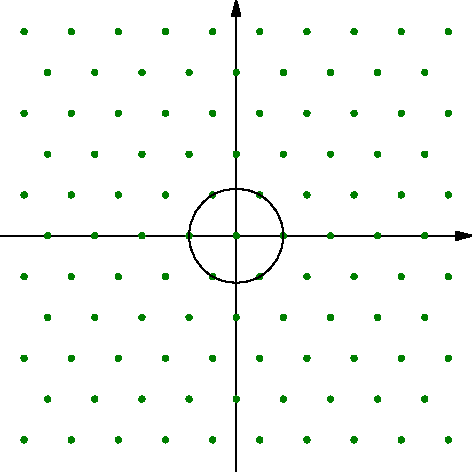
\includegraphics{./Eanneauxquad_1.pdf}
  % Eanneauxquad_1.pdf: 0x0 pixel, 300dpi, 0.00x0.00 cm, bb=
  \caption{Réseau de points d'affixes dans $\Z[j]$}
  \label{fig:Eanneauxquad_1}
\end{figure}

\begin{enumerate}
  \item Soit $x\in \R$, montrer qu'il existe $a\in \Z$ tel que $|x-a|\leq \frac{1}{2}$.
  \item On suppose que $\Z[\alpha]$ vérifie la propriété d'approximation suivante:
  \begin{displaymath}
    \forall w \in \C, \; \exists w_{\alpha} \in \Z[\alpha]\;\text{ tel que } \left| w - w_{\alpha}\right|^2 < 1
  \end{displaymath}
  Montrer que $\Z[\alpha]$ admet une division euclidienne.
  \item 
  \begin{enumerate}
    \item Montrer que pour tout $w\in \C$, il existe $x$ et $y$ réels tels que $w = x + y\alpha$.
    \item Montrer que pour tout $w\in \C$, il existe $w_{\alpha}\in \Z[\alpha]$ tel que 
    \begin{displaymath}
      |w-w_{\alpha}|^2 \leq \frac{1 + |p| + |q|}{4} 
    \end{displaymath}
    \item Montrer que les anneaux $\Z[i]$, $\Z[j]$, $\Z[i\sqrt{2}]$ admettent des divisions euclidiennes.
  \end{enumerate}
  \item 
  \begin{enumerate}
    \item Ici $\alpha$ est le nombre complexe de partie imaginaire positive vérifiant $\alpha^2 = \alpha - 2$.\newline
  Montrer que $\Z[\alpha]$ admet une division euclidienne en justifiant d'abord que, pour tout nombre complexe $w$ de partie réelle $x$ et de partie imaginaire $y$ et tous $u$ et $v$ entiers, 
\begin{displaymath}
  \left| w -(u+v\alpha)\right|^2
  = \left( x-\frac{v}{2}- u\right)^2 + \frac{7}{4}\left( \frac{2y}{\sqrt{7}}- v\right)^2  
\end{displaymath}
    \item Inspirez vous de la question précédente pour montrer que $\Z[\alpha]$ admet une division euclidienne lorsque $\alpha$ est le nombre complexe de partie imaginaire positive vérifiant $\alpha^2 = \alpha - 3$.
  \end{enumerate}
\end{enumerate}

\subsection*{IV. Applications}
Dans toute cette partie $\Z[\alpha]$ est supposé euclidien. Deux éléments $z$, $z'$ sont dits \emph{étrangers} si et seulement si $\mathcal{D}(z)\cap \mathcal{D}(z') = I$ (ensemble des inversibles).
\begin{enumerate}
  \item Dans $\Z[\alpha]$, on considère deux éléments $a_0$ et $a_1$ avec $0< |a_1|^2 < |a_0|^2$. Présenter l'algorithme d'Euclide dans ce cadre. Soit $\delta$ le dernier reste non nul renvoyé par l'algorithme, justifier qu'il se termine et que $\mathcal{D}(a_0)\cap \mathcal{D}(a_1) = \mathcal{D}(\delta)$.
  \item On se place dans l'anneau euclidien $\Z[i]$. Reproduire et compléter le tableau suivant présentant le début d'un algorithme d'Euclide étendu
  \begin{center}
\begin{tabular}{|l|l|l|l|l|} \hline
$N$ & $145$  & $34$  & . & .\\ \hline
$a$ & $8+9i$ & $5+3i$& . & .\\ \hline
$q$ &        & $2+i$ & . & .\\ \hline
$u$ & $1$    & $0$   & . & .\\ \hline
$v$ & $0$    & $1$   & . & .\\ \hline
  \end{tabular}
  \end{center}
  On pourra utiliser librement dans la suite du problème que, dans un anneau euclidien $\Z[\alpha]$, l'algorithme d'Euclide étendu initialisé par $a_0$ et $a_1$ renvoie des éléments $\delta, u, v$ de $\Z[\alpha]$ tels que $\delta = u a_0 + va_1$.
  
  \item On se place dans un anneau $\Z[\alpha]$ euclidien. Montrer que deux éléments $a_0$, $a_1$ sont étrangers si et seulement si il existe $u$ et $v$ dans $\Z[\alpha]$ tels que $ua_0 + va_1 = 1$. Formuler et prouver le théorème de Gauss valable dans ce cadre.
  
  \item On suppose $x$ et $y$ dans $\Z$ tels que $x^2 + 2 = y^3$. En utilisant l'anneau euclidien $\Z[i\sqrt{2}]$, on va montrer qu'il existe seulement deux couples solutions.
  \begin{enumerate}
    \item  Montrer que $x$ est impair.
    \item Montrer que $2i\sqrt{2}$ et $x-i\sqrt{2}$ sont étrangers. En déduire que $x+i\sqrt{2}$ et $x-i\sqrt{2}$ sont étrangers.
    \item Montrer qu'il existe un nombre fini d'irréductibles $z_1, \cdots, z_p$ deux à deux étrangers et des naturels non nuls $m_1,\cdots m_p$ tels que 
    \begin{displaymath}
      y = u z_1^{m_1}\cdots z_p^{m_p} \; \text{ avec } u \text{ inversible}
    \end{displaymath}
    Le caractère euclidien de l'anneau est-il important dans le raisonnement?
    \item Montrer qu'il existe $a$ et $b$ dans $\Z$ tels que $x+i\sqrt{2}=(a+ib\sqrt{2})^3$. Le caractère euclidien de l'anneau est-il important dans le raisonnement?
    \item Montrer que l'équation admet seulement deux couples solutions.
  \end{enumerate}
  \item On se place cette fois dans l'anneau $\Z[i\sqrt{26}]$.
  \begin{enumerate}
    \item Montrer que $3$, $1+i\sqrt{26}$, $1-i\sqrt{26}$ sont irréductibles.
    \item Que vaut $(1+i\sqrt{26})\times (1-i\sqrt{26})$ ? \newline
    Pour autant, $1+i\sqrt{26}$ est-il un cube dans $\Z[i\sqrt{26}]$ ?
  \end{enumerate} 
\end{enumerate}
